\documentclass[tikz,border=2pt]{standalone}
\usepackage{newtxtext}
\usepackage{pgfplots}
\pgfplotsset{compat=1.18}
\usetikzlibrary{patterns}

\newcommand{\bparam}{b}
\newcommand{\cparam}{c}

\begin{document}
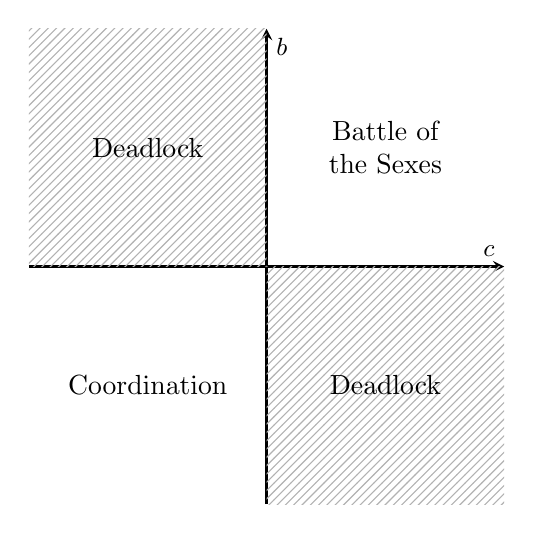
\begin{tikzpicture}
    \begin{axis}[
        width=3in,
        height=3in,
        axis x line=middle,
        axis y line=middle,
        axis line style={thick},
        xlabel={$\cparam$},
        ylabel={$\bparam$},
        xmin=-2, xmax=2,
        ymin=-2, ymax=2,
        xtick={0},
        ytick={0},
        tick label style={font=\small},
        label style={font=\small},
        enlargelimits=false,
        clip=false
    ]
    % Dominance-solvable quadrants (hatched), analogous to PD/Deadlock
    \fill[pattern=north east lines, pattern color=gray!60]
         (axis cs:0,0) -- (axis cs:-2,0) -- (axis cs:-2,2) -- (axis cs:0,2) -- cycle;
    \fill[pattern=north east lines, pattern color=gray!60]
         (axis cs:0,0) -- (axis cs:2,0) -- (axis cs:2,-2) -- (axis cs:0,-2) -- cycle;
    % Quadrant labels
    \node[align=center] at (axis cs:1,1)
        {\normalsize Battle of\\the Sexes};
    \node[align=center] at (axis cs:-1,1)
        {\normalsize Deadlock};
    \node[align=center] at (axis cs:-1,-1)
        {\normalsize Coordination};
    \node[align=center] at (axis cs:1,-1)
        {\normalsize Deadlock};
    \end{axis}
\end{tikzpicture}
\end{document}
